% ----------------------------- %
% Paper for SEXI2013            %
% http://sexi2013.org/          %
% ----------------------------- %
% Full paper:     Nov 30, 2012  %
% Notification:   Dec 17, 2012  %
% Camera-ready:   Feb  5, 2013  %
% ----------------------------- %
% Maximum pages: 2              %
% ----------------------------- %

\documentclass[runningheads,a4paper]{llncs}
\usepackage[T1]{fontenc}
\usepackage[utf8]{inputenc}


% References
\usepackage[pdftex,urlcolor=black,colorlinks=true,linkcolor=black,citecolor=black]{hyperref}
\usepackage[capitalise,nameinlink]{cleveref}
\crefname{subsection}{Subsection}{Subsections}

\usepackage{graphicx}
\usepackage{caption}
\usepackage{subcaption}

% Better typography
\usepackage[activate=compatibility]{microtype}

% Todo macro
\usepackage{color}
\newcommand{\todo}[1]{\noindent\textcolor{red}{{\bf \{TODO} #1{\bf \}}}}

% Keywords command
\newcommand{\keywords}[1]{\par\addvspace\baselineskip
\noindent\keywordname\enspace\ignorespaces#1}

\begin{document}

\mainmatter

\title{Identifying {\scshape vhs} Recording Artifacts\\
in the Age of Online Video Platforms}

\titlerunning{Identifying {\scshape vhs} Recording Artifacts}
\authorrunning{Identifying {\scshape vhs} Recording Artifacts}

\author{Thomas Steiner\inst{1} \and
        Seth van Hooland\inst{2} \and
        Ruben Verborgh\inst{3}\and
        Joseph Tennis\inst{4}}

\institute{
Universitat Politècnica de Catalunya -- Department {\scshape lsi}\\
  \urldef{\emails}\path|tsteiner@lsi.upc.edu|\emails\\
\and
Université Libre de Bruxelles -- Information and Communication Science Dept.\\
     \urldef{\emails}\path|svhooland@ulb.ac.be|\emails\\
\and
Ghent University -- iMinds -- Multimedia Lab\\
  \urldef{\emails}\path|ruben.verborgh@ugent.be|\emails\\
\and
Information School -- University of Washington\\
  \urldef{\emails}\path|jtennis@uw.edu|\emails\\
}

\maketitle

% Ignore affiliation note numbers: start footnotes from the beginning.
\setcounter{footnote}{0}

\begin{abstract}
In this position paper, we describe how analogue recording artifacts
stemming from digitized {\scshape vhs} tapes such as
grainy noises, ghosting, or synchronization issues
can be identified at Web-scale via crowdsourcing
in order to filter out content digitized by amateurs.
\end{abstract}

\keywords{Amateur Video Digitization, Video Home System~({\scshape vhs}), Long tail of niche content}

\section{Introduction}
Online video is one of the fastest growing Internet industries.
With the latest statistics of a~well-known online video
platform\footnote{\url{http://www.youtube.com/t/press_statistics}}
of 72 uploaded hours of video per minute,
it becomes evident that efficient search, recommendation, and
navigation capabilities are required in order to use 
video platforms in a~meaningful way. 
Common online video platforms typically allow their users
(i)~to search for content based on full-text query terms
that are matched against textual descriptions
of the video like its title or description,
or (ii)~to browse the archive of a~platform by category or channel,
usually based on video tags.
Users are presented a~top-$n$ ranked list of videos
that match a~given category
or query term, ranked by ranking criteria such as
\emph{relevancy}, \emph{view count},
\emph{user rating}, or \emph{upload date}.
The default ranking criteria normally being
\emph{relevancy}---a~platform-specific \emph{black box}
ranking criterium---advanced and frequently returning power-users
may prefer more transparent and traceable ranking criteria
such as the popularity-based \emph{view count}
and \emph{user rating}, or the stack-based
{\scshape lifo} (last in, first out) ranking criterium \emph{upload date}.

In this position paper, we suggest a~computer vision-based
approach to automatically filter out {\scshape vhs} content 
which has been digitized in a non-professional manner. 
Typically, this type of niche content was uploaded to the web
in the early to mid 2000s and is formally characterized by 
analogue recording artifacts stemming from {\scshape vhs} tapes. 
Common issues with digitized {\scshape vhs} videos include 
ghosting (\autoref{fig:ghosting}),
color-specific degradation,
brightness and color channel interferences,
chaotic line shift at the end of frames,
and wide horizontal noise strips (\autoref{fig:distortion}).

\section{Problem Statement}
The publication of online content produced by amateurs has received a substantial amount 
of attention. This position papers wants to raise the question to what extent 
the identification of content {\scshape digitized by amateurs} can offer a useful parameter 
to make sense out of the fast-paced growing corpus of online video. 
Exploiting the fact that an individual invested time and resources into the 
digitization of content from a {\scshape vhs} tape can hold a unique value 
both for information retrieval and research purposes. 
Especially in the context of the long tail of niche content,
automatically identifying {\scshape vhs content digitized by amateurs}     
can help to identify more quickly unique content items.
Uploaders of this type of content occasionally add tags 
such as "vintage" or "retro" but these practices are incoherent. 
Automated means to aggregate this type of content are needed 
and therefore this position paper propose a~scalable, crowdsourced way
to identify amateurishly digitized videos.

\vspace{-1em}

\begin{figure}
  \centering
  \begin{subfigure}[b]{0.45\linewidth}
    \centering
    
\includegraphics[width=\textwidth]{ghosting.png} 
    \caption{Ghosting
    [\url{http://goo.gl/NXJzw}]}
     \label{fig:ghosting}
  \end{subfigure}
  \begin{subfigure}[b]{0.45\linewidth}
    \centering
    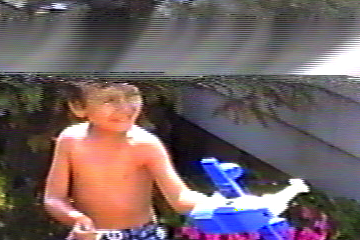
\includegraphics[width=\textwidth]{distortion.png} 
    \caption{Distortion
    [\url{http://goo.gl/zRiEQ}]}
     \label{fig:distortion}
  \end{subfigure}  
  \label{fig:artifacts}
  \caption{Typical {\scshape vhs} artifacts after amateurish digitalization.}
\end{figure}

\vspace{-3em}

\section{Methodology}

In~\cite{steiner2011crowdsourcing}, we have introduced
a~generic crowdsourcing framework for the automatic and scalable
annotation of HTML5 video:
while a~user watches a~video, the framework in the background
unobtrusively annotates it, \emph{e.g.}, as demonstrated
in the concrete case, to extract events.
The annotation framework being generic,
we can imagine a~video denoising algorithm
as presented by Yang in~\cite{yang2009videonoise}
being applied to a~video that is currently played
to detect if it suffers from {\scshape vhs} artifacts.
Over time, \emph{individual} users watching low quality digitized videos
create enough signals to eventually filter out the corpus of 
content digitized by amateurs.

\vspace{-0.5em}

\section{Conclusion}

In this position paper, we have presented a~crowdsourced,
scalable approach to detect {\scshape vhs} digitization artifacts,
where users by watching videos do useful work such as 
detecting {\scshape vhs} artifacts as a~by-product,
and thus over time allowing video platforms to filter out
a specific type of niche content by leveraging the crowd.

\vspace{-0.5em}

\footnotesize
\bibliographystyle{splncs03}
\bibliography{references}

\end{document}
